% Preamble
\documentclass{aastex631}
\usepackage{natbib}
\usepackage{latexsym}
\usepackage{graphicx}
\usepackage{epsfig}
\usepackage{amssymb}
\usepackage{amsmath}
\usepackage{epstopdf}
\usepackage{hyperref}

%%%% Custom commands
\newcommand{\gradrad}{\ensuremath{\nabla_{\rm{rad}}}}
\newcommand{\gradad}{\ensuremath{\nabla_{\rm{ad}}}}
\newcommand{\justgrad}{\ensuremath{\nabla}}
\newcommand{\delp}{\ensuremath{\delta_{\rm{p}}}}
\newcommand{\Fbot}{\ensuremath{F_{\rm{bot}}}}
\newcommand{\Ftot}{\ensuremath{F_{\rm{tot}}}}
\newcommand{\Frad}{\ensuremath{F_{\rm{rad}}}}
\newcommand{\Fconv}{\ensuremath{F_{\rm{conv}}}}
\newcommand{\Fcz}{\ensuremath{F_{\rm{cz}}}}
\newcommand{\mP}{\ensuremath{\mathcal{P}}}
\newcommand{\mD}{\ensuremath{\mathcal{D}}}
\newcommand{\dP}{\ensuremath{\delta_{\rm{p}}}}
\newcommand{\Lcz}{\ensuremath{L_{\rm{cz}}}}
\newcommand{\mR}{\ensuremath{\mathcal{R}}}
\newcommand{\mS}{\ensuremath{\mathcal{S}}}
\newcommand\Pran{\ensuremath{\mathrm{Pr}}}
\newcommand{\brunt}{Brunt-V\"{a}is\"{a}l\"{a}}

\newcommand{\angles}[1]{\langle #1 \rangle}
\newcommand{\pd}[1]{\partial_{#1}}
\renewcommand{\vec}[1]{\boldsymbol{#1}}
\newcommand{\M}[1]{\mathbf{#1}}
\renewcommand{\dot}{\vec{\cdot}}
\renewcommand{\bar}[1]{\overline{#1}}
\newcommand{\grad}{\vec{\nabla}}
\newcommand{\cross}{\vec{\times}}
\newcommand{\laplacian}{\nabla^2}

%%%% Journal preamble
\received{}
\revised{}
\accepted{}
\published{}
\submitjournal{ApJ}

\shorttitle{Convective Penetration}
\shortauthors{Anders et al}


\begin{document}

%%%% Title and Abstract
\title{Convective penetration probably parameterizes convective overshoot}
\author[0000-0002-3433-4733]{Evan H. Anders}
\affiliation{CIERA, Northwestern University, Evanston IL 60201, USA}
\author[0000-0001-5048-9973]{Adam S. Jermyn}
\affiliation{Center for Computational Astrophysics, Flatiron Institute, New York, NY 10010, USA}
\author[0000-0002-7635-9728]{Daniel Lecoanet}
\affiliation{CIERA, Northwestern University, Evanston IL 60201, USA}
\affiliation{Department of Engineering Sciences and Applied Mathematics, Northwestern University, Evanston IL 60208, USA}
\author[0000-0001-8935-219X]{Benjamin P. Brown}
\affiliation{Department Astrophysical and Planetary Sciences \& LASP, University of Colorado, Boulder, CO 80309, USA}

\correspondingauthor{Evan H. Anders}
\email{evan.anders@northwestern.edu}

\begin{abstract}
Convection is a crucial heat transport and dynamical excitation mechanism in stars.
Parameterizations like mixing length theory adequately describe bulk convective flows, but the behavior of convective motions near convective boundaries are not well understood.
In this paper we examine how convective motions mix the background thermodynamic profiles and in turn extend the size of the convection zone, a process referred to as convective penetration.
We use a simplified Boussinesq model of stellar convection with a radiative flux.
We derive a ``penetration parameter'' $\mathcal{P}$ which compares how drastically the radiative gradient deviates from the adiabatic gradient on either side of the convective boundary.
Following \citet{roxburgh1989} and \citet{zahn1991}, we derive a parameterization in which the size of the convection zone is set by $\mP$ and the energy dissipation.
We perform 3D numerical simulations using Dedalus and find good agreement with this theory.
In stellar contexts, we expect $\mathcal{P} \approx 1$ and in this regime our results suggest that convection zones may extend beyond the Schwarzschild boundary by some 20-30\% of a mixing length.
We present a MESA solar model which uses our parameterization of convective penetration, and find that the base of the solar convection zone extends by (X amount for some choice of parameters).
We briefly discuss future experiments which could verify and extend these results to stellar contexts.
\end{abstract}
\keywords{UAT keywords}



%%%% Body of paper
\section{Introduction}
\label{sec:introduction}
Convection is a crucial heat transport mechanism in stars \citep{woosley_etal_2002, hansen_etal_2004, christensen-dalsgaard_2021}, and convective dynamics influence many poorly-understood stellar phenomena.
For example, convection drives the magnetic dynamo of the Sun, leading to the host of emergent phenomena known as solar activity \citep{brun_browning_2017}.
Convection also mixes stars compositionally, which can modify observed surface abundances or inject additional fuel into convective cores, thereby extending stellar lifetimes \citep{salaris_cassisi_2017}.
Furthermore, convective motions excite waves, which can be observed and used to constrain the thermodynamic structure of stars \citep{aerts2010, basu2016}.
A complete and nuanced understanding of convection is therefore crucial for understanding stellar structure, evolution, and observations.

Despite decades of study, robust parameterizations for the mechanisms broadly referred to as ``convective overshoot'' remain elusive, and improved parameterizations could resolve many discrepancies between observations and structure models.
In the stellar structure literature, ``convective overshoot'' refers to any convectively-driven mixing which occurs beyond the boundaries of the unstable convection zone.
This mixing can influence, for example, observed surface lithium abundances in the Sun and solar-type stars which align poorly with models \citep{pinsonneault1997, carlos_etal_2019, dumont_etal_2021}.
Furthermore, modern spectroscopic observations suggest a lower solar metallicity than previously thought, and models computed with modern metallicity estimates and opacity tables have shallower convection zones than helioseismic observations suggest \citep{basu_antia_2004, bahcall_etal_2005, bergemann_serenelli_2014, vinyoles_etal_2017, asplund_etal_2021}; modeling and observational discrepancies can be reduced with additional mixing below the convective boundary \citep{christensen-dalsgaard_etal_2011}.
There is also ample evidence from massive stars with core convection that currently-employed prescriptions of convective overshoot are inadequate \citep{claret_torres_2018, jermyn_etal_2018, viani_basu_2020, martinet_etal_2021, pedersen_etal_2021}.
Since core convective overshoot increases the reservoir of fuel available for nuclear fusion at each stage in stellar evolution, improved models of core convective boundary mixing could have profound impacts on the post-main sequence evolution and remnant formation of massive stars \citep{farmer_etal_2019, higgins_vink_2020}.
In order to ensure that models can be evolved on fast (human) timescales, 1D stellar evolution codes rely on simple parameterizations of convection \citep[e.g., mixing length theory,][]{bohm-vitense1958} and convective overshoot \citep{shaviv_salpeter_1973, maeder1975, herwig2000, paxton_etal_2011, paxton_etal_2013, paxton_etal_2018, paxton_etal_2019}.
While some preliminary work has been done to couple 3D dynamical convective simulations with 1D stellar evolution codes \citep{jorgensen_weiss_2019}, these calculations are currently prohibitively expensive to perform e.g., at every timestep in a stellar evolution calculation.
In short, in order to resolve many of the discrepancies between current stellar evolution models and observations, we must come to a more complete, and \emph{parameterizeable} understanding of the manner in which convective motions extend beyond convective boundaries.

The mechanisms referred to as ``convective overshoot'' in the stellar literature fall into two hydrodynamical classes.
The first class is, confusingly, also called ``\emph{convective overshoot}'' in the fluid dynamics literature and refers to motions which extend beyond the convective boundary and mix chemical compositions but importantly do not adjust the thermodynamic profile.
The second class is called ``\emph{convective penetration},'' and refers to convective motions which mix the thermodynamic profiles beyond the convective boundary, thereby extending the adiabatically-mixed convective region.
We will follow a deep history \citep{zahn1991, brummell_etal_2002, korre_etal_2019} and use this terminology; the primary focus of this work is convective penetration.

Convective overshoot and penetration have been studied in the laboratory and through numerical simulations for decades, and the state of the field has been regularly reviewed \citep[e.g.,][]{marcus_etal_1983, zahn1991, browning_etal_2004, rogers_etal_2006, viallet_etal_2015, korre_etal_2019}.
One parameter which is commonly linked to penetration or overshoot is the ``stiffness'' of the radiative-convective interface; the stiffness is a ratio which states how stable a radiative zone is compared to an adjacent convection zone according to some measure like a dynamical frequency or characteristic entropy gradient.
Experiments and simulations exhibiting extensive convective penetration in water or other simplified, Boussinesq setups have a long history \citep{ musman1968, deardorff_etal_1969, moore_weiss_1973}.
Some of these recent simplified studies suggest that the penetration depth is highly dependent on the stiffness of the radiative-convective interface \citep{couston_etal_2017, toppaladoddi_wettlaufer_2018}, and some find very little penetration but significant stiffness-dependent overshoot \citep{korre_etal_2019}.
Some studies in density-stratified or fully compressible, stratified systems \citep[e.g.,][]{hurlburt_etal_1986, saikia_etal_2000} also found significant penetration depths, with multiple authors finding results suggesting that both penetration and overshoot depths were determined by the stiffness \citep{hurlburt_etal_1994, singh_etal_1995, browning_etal_2004, dietrich_wicht_2018}.
However, some studies have contradicted these results, showing little to no dependence on the stiffness \citep{brummell_etal_2002, rogers_glatzmaier_2005}.
Many modern simulations utilize stellar structure models as background states and find significant convective overshoot and/or penetration \citep{browning_etal_2004, rogers_etal_2006, kitiashvili_etal_2016, brun_etal_2017, pratt_etal_2017, higl_etal_2021}.
This host of experiments indeed suggests that convective penetration is \emph{probably} a process that happens in stars, but no clear model has emerged which explains whether convective penetration depends on stiffness or some other quantity.

There are hints in the literature that convective penetration may be dependent upon energy fluxes.
\citet{roxburgh1978, roxburgh1989, roxburgh1992, roxburgh1998} derived an ``integral constraint'' from the energy conservation equation and found that a spatial integral of the flux puts and upper limit on the size of a penetrative region.
\citet{zahn1991} theorized that convective penetration should depend only on how steeply the radiative temperature gradient varies at the convective boundary.
Following \citet{zahn1991}'s work, \citet{rempel2004} derived a semianalytic model and suggested that inconsistencies seen in simulations of penetrative dynamics can be explained by the magnitude of the fluxes or luminosities driving the simulations.
Indeed, some simulations have tested this exact idea, and found that penetration depths depend strongly on the input flux \citep{singh_etal_1998, kapyla_etal_2007, tian_etal_2009, hotta2017, kapyla2019}.
Furthermore, in the limit of low stiffness, the simulations of \citet{hurlburt_etal_1994} and \citet{rogers_etal_2006} seem to agree with Zahn's theory (although at high stiffness they disagree).
In light of these results, and the possible importance of fluxes, Roxburgh's integral constraint and Zahn's theory deserve to be revisited.

In this work, we design two numerical experiments to test the idea that the penetration depth depends on the shape of the radiative gradient at the convective boundary.
We use a modified incompressible, Boussinesq model to study the simplest possible system, and derive theoretical predictions for the size of the penetrative zone.
We test this theory using 3D numerical simulations.
\begin{quote}
\emph{
We find that the extent of convective penetration depends strongly on the shape and magnitude of the radiative gradient near the convective boundary.
}
\end{quote}
Thus, the penetration depth can be calculated using the radiative conductivity (or opacity) around the convective boundary.

We present these findings as follows.
In Sec.~\ref{sec:theory}, we describe our modified Boussinesq equations, derive a theory of convective penetration, and retrieve predictions for our two experimental designs from that theory.
In Sec.~\ref{sec:simulation_details}, we describe our simulation setup and parameters.
In Sec.~\ref{sec:results}, we present the results of these simulations, with a particular focus on the depth of the penetrative regions.
In Sec.~\ref{sec:solar_model}, we create and discuss a solar MESA model which uses this theory to determine the bottom of the solar convection zone.
Finally, we discuss how future simulations can put finer constraints on this theory in Sec.~\ref{sec:discussion}.

\section{Theory}
\label{sec:theory}

\subsection{Equations \& flux definitions}
\label{sec:theory_equations}
Throughout this work, we will utilize a modified version of the incompressible Boussinesq equations of motion,
\begin{align}
&\grad\dot\vec{u} = 0 
\label{eqn:incompressible} \\
&\partial_t \vec{u} + \vec{u}\dot\grad\vec{u} = -\frac{1}{\rho_0}\grad p + \frac{\rho_1}{\rho_0}\vec{g} + \nu\grad^2 \vec{u} 
\label{eqn:momentum} \\
&\partial_t T + \vec{u}\dot\grad T + w \gradad + \grad\dot[-k \grad \overline{T}] = \chi\grad^2 T' + Q
\label{eqn:temperature} \\
&\frac{\rho_1}{\rho_0} = -|\alpha| T.
\label{eqn:boussinesq}
\end{align}
Here, the density is decomposed into a constant background $\rho_0$ with fluctuations $\rho_1$ which appear only in the buoyancy force and depend on the temperature $T$ and the coefficient of thermal expansion $\alpha = \partial\ln\rho / \partial T$.
We furthermore define the velocity vector $\vec{u}$, the viscous diffusivity $\nu$, the thermal diffusivity $\chi$, the bulk internal heating $Q$ \citep[similar but not identical to that described in e.g.,][]{goluskin2016}, the adiabatic gradient $\gradad$, and a height-dependent thermal conductivity $k$.
We will consider Cartesian coordinates $(x, y, z)$ with a constant vertical gravity $\vec{g} = -g\hat{z}$.
Throughout this work, we will represent horizontal averages with bars ($\overline{\,\cdot\,}$) and fluctuations away from those averages with primes ($'$).
Thus, in Eqn.~\ref{eqn:temperature}, $\bar{T}$ is the horizontally averaged temperature and $T'$ are fluctuations away from that; both of these fields evolve in time according to this equation.

Assuming convection reaches a time-stationary state, the fluxes are found by horizontally-averaging then vertically integrating Eqn.~\ref{eqn:temperature} to find
\begin{equation}
\overline{\Ftot} = \overline{\Frad} + \overline{\Fconv} = \int Q dz + \Fbot,
\label{eqn:flux_definition}
\end{equation}
where $\Fbot$ is the flux carried at the bottom of the domain, and $\overline{\Ftot}$ is the total flux, which can vary in height due to the heating $Q$.
We allow the mean temperature profile $\overline{T}$ to carry a radiative flux $\bar{\Frad} = -k \grad \overline{T}$.
We note that $k$ and $-\partial_z \bar{T}$ fully specify $\bar{\Frad}$ and in turn the convective flux, $\bar{\Fconv} = \bar{\Ftot} - \bar{\Frad}$.
We define the gradient and radiative gradient 
\begin{equation}
\justgrad \equiv -\partial_z \bar{T} \qquad
\gradrad \equiv \frac{\bar{\Ftot}}{k}.
\label{eqn:gradrad_definition}
\end{equation}
We have defined the $\justgrad$'s as positive quantities to align with stellar structure conventions.
Marginal stability is achieved when $\justgrad = \gradad$, a constant.
We note that the classical Schwarzschild boundary of the convection zone is the height $z = L_s$ at which $\gradrad = \gradad$ and $\bar{\Fconv} = 0$.

The addition of a nonzero $\gradad$ to Eqn.~\ref{eqn:temperature} was derived by \citet{spiegel_veronis_1960} and utilized by e.g., \citet{korre_etal_2019}.
In this work, we have decomposed the radiative diffusivity into a background portion ($\grad\dot \bar{\Frad}$) and a fluctuating portion ($\chi \grad^2 T'$); by doing so, we have introduced a height-dependent $\gradrad$ to the equation set while preserving the diffusive behavior on fluctuations felt by classical Rayleigh-B\'{e}nard convection.
Here, we will assume a model in which an unstable convection zone ($\gradrad > \gradad$) sits below a stable radiative zone ($\gradrad < \gradad$), but the same logic applies to the inverted problem.

\subsection{Kinetic energy \& the dissipation-flux link}
\label{sec:theory_energy}
\begin{figure}[t!]
\centering
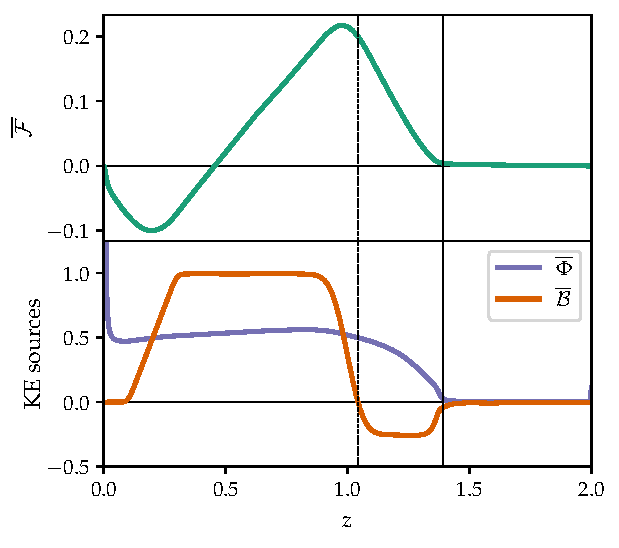
\includegraphics[width=\textwidth]{theory_profiles.pdf}
\caption{
(left) The vertical profile of the kinetic energy fluxes $\mathcal{F}$.
This profile goes to zero at the bottom boundary, again at the dashed line, and at the top of the PZ near $z \approx 1.5$; Eqn.~\ref{eqn:integral_constraint} holds between any two of these points.
(middle) the evolved value of $\justgrad$ (green) compared to $\gradad$ (grey) and $\gradrad$ (red); note the extended penetration zone where $\justgrad \approx \gradad > \gradrad$.
(right) Source terms from Eqn.~\ref{eqn:kinetic_energy_1D} normalized by the maximum of $\overline{\mathcal{B}}$.
\label{fig:theory_profiles}
}
\end{figure}

Taking an inner product of the velocity and Eqn.~\ref{eqn:momentum} reveals the kinetic energy equation,
\begin{equation}
\frac{\partial \mathcal{K}}{\partial t}
+ \grad\dot\mathcal{F}
= \mathcal{B} - \Phi,
%\frac{\partial}{\partial t}\left(\frac{|\vec{u}|^2}{2}\right) 
%+ \grad\dot\left[\vec{u}\left(\frac{|\vec{u}|^2}{2} + \frac{p}{\rho_0}\right) - \nu\vec{u}\cross\vec{\omega}\right]
%= |\alpha| g w T - \nu|\vec{\omega}|^2,
\label{eqn:kinetic_energy}
\end{equation}
where we define the kinetic energy $\mathcal{K} \equiv |\vec{u}|^2/2$, the fluxes of kinetic energy $\mathcal{F} \equiv \left[\vec{u}(\mathcal{K} + p/\rho_0) - \nu\vec{u}\cross\vec{\omega} \right]$, the buoyant energy generation rate $\mathcal{B} \equiv |\alpha| g w T'$, and the viscous dissipation rate $\Phi \equiv \nu |\vec{\omega}|^2$ where $\vec{\omega} = \grad\cross\vec{u}$ is the vorticity and $|\vec{u}|^2 = \vec{u}\dot\vec{u}$ \& $|\vec{\omega}|^2 = \vec{\omega}\dot\vec{\omega}$.
We next take a horizontal- and time-average of Eqn.~\ref{eqn:kinetic_energy} (which we will represent with $\bar{\,\cdot\,}$ for simplicity).
Assuming that $\bar{\mathcal{K}}$ reaches a statistically stationary state, convective motions satisfy
\begin{equation}
\frac{d\bar{\mathcal{F}}}{dz} = \bar{\mathcal{B}} - \bar{\Phi}.
\label{eqn:kinetic_energy_1D}
\end{equation}
It is reasonable to assume that $\mathcal{F}$ is zero at the boundaries of the convecting region (see Fig.~\ref{fig:theory_profiles}, left panel).
We integrate Eqn.~\ref{eqn:kinetic_energy_1D} vertically between these zeros of the flux to find
\begin{equation}
\int \bar{\mathcal{B}}\,dz = \int \bar{\Phi}\,dz.
\label{eqn:integral_constraint}
\end{equation}
Integral constraints of this form are the basis for a broad range of analyses in Boussinesq convection \citep[see e.g.,][]{ahlers_etal_2009, goluskin2016} and were considered in the context of penetrative stellar convection by \citet{roxburgh1989}.
Eqn.~\ref{eqn:integral_constraint} is the straightforward statement that work by buoyancy on large scales must be balanced by viscous dissipation on small scales.

We now find it instructive to break up the convecting region into a classical ``convection zone'' (CZ) and a extended ``penetration zone'' (PZ); we will assume that convective motions are efficient in each of these zones so that $\justgrad = \gradad$ in both the CZ and PZ.
We furthermore note that the buoyant energy generation is directly proportional to the convective flux, $\bar{\mathcal{B}} = |\alpha|g\bar{w T'} = |\alpha| g \bar{\Fconv}$.
Thus, in the PZ where $\gradad > \gradrad$, we know that $\bar{\Fconv} < 0$ and so $\bar{\mathcal{B}} < 0$ too (see the discussion around Eqn.~\ref{eqn:gradrad_definition}).
Breaking up Eqn.~\ref{eqn:integral_constraint}, we see that
\begin{equation}
\int_{\rm{CZ}} \bar{\mathcal{B}}\,dz \qquad=\qquad
\int_{\rm{CZ}} \bar{\Phi}\,dz + \int_{\rm{PZ}} \bar{\Phi}\,dz + \int_{\rm{PZ}}(-\bar{\mathcal{B}})\,dz.
\label{eqn:constraint_cz_pz_split}
\end{equation}
Eqn.~\ref{eqn:constraint_cz_pz_split} is thus arranged so that the (positive) buoyant engine of convection is on the left-hand side, and the (positive) sinks of work are on the RHS.
We see that the size of the PZ is set by some combination of viscous dissipation and buoyancy breaking.
We now parameterize the fraction of the buoyant engine consumed by CZ dissipation  
\begin{equation}
f \equiv \frac{\int_{\rm{CZ}} \bar{\Phi}\,dz}{\int_{\rm{CZ}}\bar{\mathcal{B}}\,dz}.
\label{eqn:f_defn}
\end{equation}
Under this parameterization, Eqn.~\ref{eqn:constraint_cz_pz_split} can be written
\begin{equation}
\frac{\int_{\rm{PZ}} \bar{\Phi}\,dz + \int_{\rm{PZ}}(-\bar{\mathcal{B}})\,dz}{\int_{\rm{CZ}} \bar{\mathcal{B}}\,dz}
= 1 - f,
\label{eqn:first_pz_parameterization}
\end{equation}
and we can immediately read off limits on a hypothetical PZ according to $f$,
\begin{enumerate}
\item In the limit that $f \rightarrow 0$, viscous dissipation is extremely inefficient.
It is probably also reasonable to assume that $\int_{\rm{PZ}}\bar{\Phi}\,dz \rightarrow 0$, and so Eqn.~\ref{eqn:first_pz_parameterization} states that the PZ must be large enough for its negative buoyant work to be equal in magnitude to the positive buoyant work of the CZ.
This is the integral constraint on the maximum size of the PZ that \citet{roxburgh1989} derived.
\item In the limit that $f \rightarrow 1$, viscous dissipation is efficient in the CZ and cancels out the work done by buoyancy.
This is the case in standard Rayleigh-B\'{e}nard convection when the convection is contained between two hard plates.
Per Eqn.~\ref{eqn:first_pz_parameterization}, the positive-definite PZ terms must approach zero and no PZ develops in this limit.
\end{enumerate}
In general, we anticipate from the results of e.g., \citet{currie_browning_2017} that $f$ is closer to 1 than 0, but its precise value must be measured directly from simulations.
Indeed, we find that $f \gg 0$ but $f < 1$ in our simulations (see e.g., Fig.~\ref{fig:theory_profiles}, right panel).

Assuming that a PZ of depth $\delp$ develops above a CZ of depth $L_{\rm{CZ}}$, we model the PZ dissipation as
\begin{equation}
\int_{\rm{PZ}} \bar{\Phi}\,dz = \xi\frac{\delp}{L_{\rm{CZ}}}\int_{\rm{CZ}}\bar{\Phi} = \xi \delp \Phi_{\rm{CZ}}.
\label{eqn:xi_defn}
\end{equation}
Here $\Phi_{\rm{CZ}}$ is the average dissipation value in the CZ and $\xi$ is a parameter that describes the shape of the dissipation profile as a function of height in the PZ.
In other words, we assume that $\bar{\Phi} \approx \Phi_{\rm{CZ}}$ at the CZ-PZ boundary and then falls off with height.
The shape of $\bar{\Phi}$ determines the value of $\xi$, with a linear falloff producing $\xi = 1/2$, a quadratic falloff producing $\xi = 2/3$, and if $\bar{\Phi}$ does not decline with height then $\xi = 1$.
Regardless, $\xi$ is another measurable parameter bounded by $[0, 1]$. 
With this parameterization, we rewrite Eqn.~\ref{eqn:first_pz_parameterization}
\begin{equation}
-\frac{\int_{\rm{PZ}}\bar{\Fconv}\,dz}{\int_{\rm{CZ}}\bar{\Fconv}\,dz} + f\xi\frac{\delp}{L_{\rm{CZ}}}
= (1 - f).
\label{eqn:theory_fraction}
\end{equation}
In order to derive a specific prediction for the PZ depth, it is necessary to specify the vertical shape of $\overline{\Fconv}$.
We will study two cases in this work, laid out below.
In both of these cases, we will define a nondimensional ``Penetration Parameter'' whose magnitude is set by the ratio of the convective flux some equidistant length $\epsilon$ both above and below the Schwarzschild convective boundary $L_s$ (assuming the region above the boundary is an adiabatic penetrative zone),
\begin{equation}
\mP \equiv -\frac{\overline{\Fconv}(z = L_s - \epsilon)}{\overline{\Fconv}(z = L_s + \epsilon)}.
\label{eqn:theory_P_defn}
\end{equation}
Since $\Fconv < 0$ in the PZ, the sign of $\mP$ is positive.
Intuitively, $\mP$ describes which terms are important in Eqn.~\ref{eqn:first_pz_parameterization}.
When $\mP \ll 1$, the buoyancy term dominates in the PZ and dissipation can be neglected there.
When $\mP \gg 1$, buoyancy is negligible in the PZ and dissipation constrains the size of the PZ.
When $\mP \sim 1$, both terms matter.



\subsubsection{Case I: Discontinuous flux}
\label{sec:discontinuous_theory}
We first consider a model which satisfies
\begin{equation}
\overline{\Fconv}(z) = \Fcz \begin{cases}
1			&	z \leq \Lcz,\\
-\mP_D^{-1}  & 	z > \Lcz 
\end{cases}.
\end{equation}
Here, $\Fcz$ is a constant value of flux carried in the convection zone and $\mP_D$ is the penetration parameter (subscript D for discontinuous case).
Plugging this functional form of the flux into Eqn.~\ref{eqn:theory_fraction}, and integrating the CZ over a depth $L_{\rm{CZ}}$ below $L_s$ and the PZ over a depth $\delp$ above $L_s$, we predict
\begin{equation}
\frac{\delp}{L_{\rm{CZ}}} = \mP_D \frac{1 - f}{1 + \xi f \mP_D}.
\label{eqn:discontinuous_prediction}
\end{equation}
Assuming that $f$ is a weak function of $\mP_D$, we see that the size of the penetration region is roughly linearly proportional to $\mP_D$ at small $\mP_D$, but saturates due to dissipation at large $\mP_D$.
Intuitively, this result makes sense: as $\mP_D$ grows, the magnitude of $\overline{\Fconv}$ and the breaking force of buoyancy in the PZ shrink, resulting in larger penetrative regions (but this growth cannot extend indefinitely).

\subsubsection{Case II: Piecewise linear flux}
\label{sec:linear_theory}
We next assume that $\overline{\Fconv}(z)$ is not discontinuous at the CZ-PZ boundary, but that its derivative may be,
\begin{equation}
\overline{\Fconv}(z) = 
\frac{\partial \Frad}{\partial z}\bigg|_{\rm{CZ}}
\begin{cases}
(L_p - z) & z \leq L_p \\
-\mP_L^{-1} (z - L_p) & z > L_p
\end{cases},
\end{equation}
where $(\partial \Frad / \partial z)|_{\rm{CZ}}$ is a constant and $\mP_L$ is the penetration parameter (subscript L for linear case).
Again, solving Eqn.~\ref{eqn:theory_fraction} with this functional form of the flux and integrating over $L_{\rm{CZ}}$ in the CZ and $\delp$ in the PZ, we retrieve a quadratic equation.
This equation has two solution branches, only one of which corresponds to a positive value of $\delp$.
On that branch, we find
\begin{equation}
\frac{\delp}{L_p} = \sqrt{\mP_L (1 - f)} \,\,(\sqrt{\zeta^2 + 1} - \zeta),
\label{eqn:linear_prediction}
\end{equation}
where $\zeta \equiv (\xi f/2)\sqrt{\mP_L/(1-f)}$.
So we expect the penetration depth to be roughly proportional to $\sqrt{\mP_L}$ for small values of $\mP_L$, and to again saturate at large values of $\mP_L$. 

In this work, we will test the predictions of Eqns.~\ref{eqn:discontinuous_prediction} and \ref{eqn:linear_prediction}.
Our goals are to see if the predicted scalings with the penetration parameter $\mP$ are realized in simulations, and to measure the dependence of $f$ and $\xi$ on various parameters in local simulations.

\section{Simulation Details}
We nondimensionalize Eqns.~\ref{eqn:incompressible}-\ref{eqn:boussinesq} on the length scale of the Schwarzschild-unstable convection zone $L_s$, the timescale of freefall across that convection zone $\tau_{\rm{ff}}$, and the temperature scale of the internal heating over that freefall time $\Delta T$,
\begin{equation}
\begin{split}
&T^* = (\Delta T)T = Q_0 \tau_{\rm{ff}} T,\qquad
\partial_{t^*} = \tau_{\rm{ff}}^{-1}\partial_t = \left(\frac{|\alpha| g Q_0}{L_s}\right)^{1/3} \partial_t,\qquad
\grad^* = L_s^{-1} \grad,\qquad
\vec{u}^* = u_{\rm{ff}}\vec{u} = \left(|\alpha| g Q_0 L_s^2\right)^{1/3}\vec{u},
\\
&p^* = \rho_0 u_{\rm{ff}}^2\varpi,\qquad
k^* = (L_s^2 \tau_{\rm{ff}}^{-1})k,\qquad
Q^* = Q_0 Q,\qquad
\mR = \frac{u_{\rm{ff}} L_s}{\nu},\qquad
\Pran = \frac{\nu}{\chi}.
\end{split}
\end{equation}
For convenience, here we define quantities with $*$ (e.g., $T^*$) as being the ``dimensionful'' quantities of Eqns.~\ref{eqn:incompressible}-\ref{eqn:boussinesq}.
Going forward, quantities without $*$ (e.g., $T$) will be dimensionless.
The dimensionless equations of motion are therefore
\label{sec:simulation_details}
\begin{align}
&\grad\dot\vec{u} = 0 
\label{eqn:nondim_incompressible} \\
&\partial_t \vec{u} + \vec{u}\dot\grad\vec{u} = -\grad \varpi + T \hat{z} + \mR^{-1}\grad^2 \vec{u}
\label{eqn:nondim_momentum} \\
&\partial_t T + \vec{u}\dot\grad T + w \grad_{\rm{ad}}  + \grad\dot[-k \grad \overline{T}] = (\Pran\mR)^{-1}\grad^2 T' + Q.
\label{eqn:nondim_temperature}
\end{align}
We construct a domain in the range $z \in [0, L_z]$ where in this work we choose $L_z \geq 2$ so that the domain is at least twice as deep as the Schwarzschild-unstable convection zone.
We decompose the temperature field into a time-stationary initial background and fluctuations, $T(x, y, z, t) = T_0(z) + T_1(x, y, z, t)$.
For boundary conditions, we impose impenetrable, no-slip boundary conditions at the top and bottom of the box so that $\vec{u} = 0$ at $z = [0, L_z]$.
We also impose a fixed-flux boundary at the bottom of the box ($\partial_z T_1 = 0$ at $z = 0$) and a fixed temperature boundary at the top of the domain ($T_1 = 0$ at $z = L_z$).
For a select few simulations, we impose stress-free instead of no-slip boundary conditions ($w = 0$ and $\partial_z u = \partial_z v = 0$ at $z = [0, L_z]$).

We impose a constant internal heating which spans only part of the convection zone,
\begin{equation}
Q = \begin{cases}
0		& z < 0.1\,\,\rm{or}\,\,z\geq 0.1 + \delta_H,\\
Q_{\rm{mag}}		& 0.1 \leq z \leq 0.1 + \delta_H
\end{cases}.
\label{eqn:sim_Q}
\end{equation}
The integrated value of the flux through the system from the heating is therefore $F_H = \int_0^{L_z} Q_{\rm{mag}} dz = Q_{\rm{mag}}\delta_H$.
Throughout this work we choose $Q_{\rm{mag}} = 1$ and $\delta_H = 0.2$ so $F_H = 0.2$.
We offset this heating from the bottom boundary to $z = 0.1$ to avoid heating within the bottom impenetrable boundary layer where velocities go to zero and $k$ is small; this prevents strong temperature gradients from establishing there.
We assume that the (adiabatic) temperature gradient at the bottom boundary carries some flux, $\Fbot = \zeta F_H$ and we choose $\zeta = 10^{-3}$ so that most of the flux in the convection zone is carried by the convection.

In our equations, we expect the volume-average convective velocities to depend on the magnitude of the heating, $\angles{\vec{u}} \approx Q_{\rm{mag}}^{1/2} \approx 1$, so the characteristic convective frequency is $f_{\rm{conv}} \approx \angles{\vec{u}} L_s \approx 1$.
The stiffness is defined,
\begin{equation}
\mS \equiv \frac{N^2}{f_{\rm{conv}}^2} \approx N^2,
\end{equation}
where $N^2$ is the \brunt$\,$frequency in the radiative zone.
In our nondimensionalization, $N^2 = \gradad - \gradrad$.
We treat $\mS$ as a control parameter; by choosing a value of the stiffness we set the magnitude of $\justgrad$, which in turn sets the value of $k$ in the radiative zone.

The crucial place in which our model differs from that of prior work is that we define the ``Penetration Parameter,'' $\mP$, according to Eqn.~\ref{eqn:theory_P_defn}.
We construct our experiments so that $\mP$ and $\mS$ can be varied separately.
We suspect that many past experiments have implicitly set $\mP \approx \mS^{-1}$, and therefore found negligible penetration for moderate to high stiffness.

Aside from $\mS$ and $\mP$, the two remaining control parameters $\mR$ and $\Pran$ determine the degree of turbulence.
The value of $\mR$ roughly corresponds to the value of the peak Reynolds number $\rm{Re} = \mR |\vec{u}|$ measured in the simulations, and we set the ratio of the diffusivities $\Pran = 0.5$ throughout this work.
Astrophysical convection is in the limit of $\Pran \ll 1$ \citep{garaud2021}; we choose a modest value of $\Pran$ which slightly separates the scales between thermal and viscous structures while still allowing us to achieve convection with large Reynolds and P\'{e}clet numbers.

\subsection{Case I: Discontinuous flux}
Most of the simulations in this paper have a discontinuous convective flux at the Schwarzschild convective boundary.
We achieve this by constructing a discontinuous radiative conductivity,
\begin{equation}
k = \begin{cases}
k_{\rm{CZ}}	&	z < 1 \\
k_{\rm{RZ}} &	z \geq 1
\end{cases},
\label{eqn:sim_discontinuous_k}
\end{equation}
where CZ refers to the convection zone and RZ refers to the radiative zone (some of which will be occupied by the penetrative zone PZ).
Leaving $\mS$ and $\mP_D$ as free parameters and requiring that the adiabatic gradient can carry $\Fbot$ at $z = 0$ and that the radiative gradient can carry $F_H + \Fbot$ for $z \geq 1$ specifies this system fully,
\begin{equation}
k_{\rm{RZ}} = \frac{\delta_H}{\mS\mP_D},\qquad
k_{\rm{CZ}} = k_{\rm{RZ}}\frac{1}{1 + \zeta + \mP_D^{-1}},\qquad
\gradad = Q_{\rm{mag}}\mS\mP_D(1 + \zeta + \mP_D^{-1}),\qquad
\gradrad = \gradad - Q_{\rm{mag}}\mS.
\end{equation}

We study three sweeps through the ($\mP_D$, $\mS$, $\mR$) parameter space in this paper in which we hold two of these parameters constant and vary the other.
We study an additional sweep through $\mR$ parameter space using stress-free boundaries to compare to our no-slip cases.
We use reference values of $\mP_D = 4$, $\mS = 10^3$, and $\mR = 400$; all parameter space sweeps pass through these values.
According to Eqn.~\ref{eqn:discontinuous_prediction}, we expect $\delp \propto \mP_D$.

\subsection{Case II: Piecewise linear flux}
We additionally study a select few simulations where the flux's gradient may be discontinuous at the Schwarzschild convective boundary.
We achieve this by constructing a radiative conductivity with a piecewise discontinuous gradient,
\begin{equation}
\partial_z k = \partial_z k_0
\begin{cases}
1	&	z < 1 \\
\mP_L^{-1} &	z \geq 1
\end{cases}
\label{eqn:sim_linear_k}
\end{equation}
Since $k$ varies with height, the value of $\mS$ and $\mP$ also vary with height; we specify their values at $z = 2$.
By this choice, we require
\begin{equation}
\partial_z k_0 = \frac{\delta_H}{L_s \mS \psi},\qquad
k_b = \frac{\delta_H\zeta}{\mS\psi},\qquad
\gradad = Q \mS \psi,
\end{equation}
where $\psi \equiv 1 + \mP_L(1 + \zeta)$.
In these simulations, we hold $\mS = 10^3$ and $\mR = 800$ while varying $\mP_L$.
According to Eqn.~\ref{eqn:linear_prediction}, we expect $\delta_p \propto \mP_L^{1/2}$.

\subsection{Numerics}
We time-evolve equations \ref{eqn:nondim_incompressible}-\ref{eqn:nondim_temperature} using the Dedalus pseudospectral solver \citep{burns_etal_2020}\footnote{we use commit \href{https://github.com/DedalusProject/dedalus/commit/efb13bdaa09816dde3eee897bc2a15fc284ea2f1}{efb13bd}; the closest stable release to this commit is \href{https://github.com/DedalusProject/dedalus/releases/tag/v2.2006}{v2.2006}.} using timestepper SBDF2 \citep{wang&ruuth2008} and safety factor 0.35.
All fields are represented as spectral expansions of $n_z$ Chebyshev coefficients in the vertical ($z$) direction and as ($n_x$,$n_y$) Fourier coefficients in the horizontal ($x$,$y$) directions; our domains are therefore horizontally periodic.
The aspect ratio of our domains is two so that $x \in [0, L_x]$ and $y \in [0, L_y]$ with $L_x = L_y = 2 L_z$.
To start our simulations, we add random noise temperature perturbations with a magnitude of $10^{-3}$ to a background temperature profile $\overline{T}$; we discuss the choice of $\overline{T}$ in appendix \ref{app:accelerated_evolution}.
We produce the figures in this paper using matplotlib \citep{hunter2007, mpl3.3.4}.
All of the Python scripts used to run the simulations in this paper and to create the figures in this paper are publicly available in a git repository, found at [CITE].

Spectral methods with finite coefficient expansions cannot capture true discontinuities.
In order to approximate discontinuous functions such as Eqns.~\ref{eqn:sim_Q}, \ref{eqn:sim_discontinuous_k}, and \ref{eqn:sim_linear_k}, we must use smooth transitions.
To create these smooth transitions, we define an approximate Heaviside step function using the error function,
\begin{equation}
H(z; z_0, d_w) = \frac{1}{2}\left(1 + \rm{erf}\left[\frac{z - z_0}{d_w}\right]\right).
\label{eqn:heaviside}
\end{equation}
In the limit that $d_w \rightarrow 0$, this function behaves identically to the classical Heaviside function centered at $z_0$.
While constructing Eqn.~\ref{eqn:sim_Q} and Eqn.~\ref{eqn:sim_linear_k}, we use $d_w = 0.02$; while constructing Eqn.~\ref{eqn:sim_discontinuous_k} we use $d_w = 0.075$.
In all other cases, we use $d_w = 0.05$.

\subsection{Penetration depth measurements}
In our evolved simulations, we find that the penetrative region has a nearly adiabatic stratification $\justgrad \approx \gradad$.
In order to characterize the vertical extent of the penetrative region, we measure how drastically $\justgrad$ has departed from $\gradad$.
We define the difference between the adiabatic and radiative gradient,
\begin{equation}
\Delta\justgrad \equiv \gradad(z) - \gradrad(z).
\end{equation}
We measure penetration and overshoot depths in terms of ``departure points,'' or heights at which the realized temperature gradient $\justgrad$ has evolved away from the adiabatic $\gradad$ by some fraction $h < 1$.
Specifically,
\begin{equation}
L_s + \delta_{h} = \rm{max}(z) \mid \justgrad > \gradad - h\,\Delta\justgrad.
\label{eqn:delta_p_measures}
\end{equation}
In this work, we measure the 10\% ($\delta_{0.1}$), 50\% ($\delta_{0.5}$), and 90\% ($\delta_{0.9}$) departure points.
Using \citet{zahn1991}'s terminology, $\delta_{0.5}$ is the mean value of the top of the PZ while $\delta_{0.9} - \delta_{0.1}$ roughly represents the width of the ``thermal adjustment layer.''
We will simply refer to these as three different measures of the top of the PZ.
We find that these measurements based on the (slowly-evolving) thermodynamic profile are more robust and straightforward than many previous dynamically-based prescriptions \citep[see e.g.,][for a nice discussion]{pratt_etal_2017}.

\section{Results}
\label{sec:results}

\subsection{Qualitative description of simulation evolution}

\begin{figure}[t!]
\centering
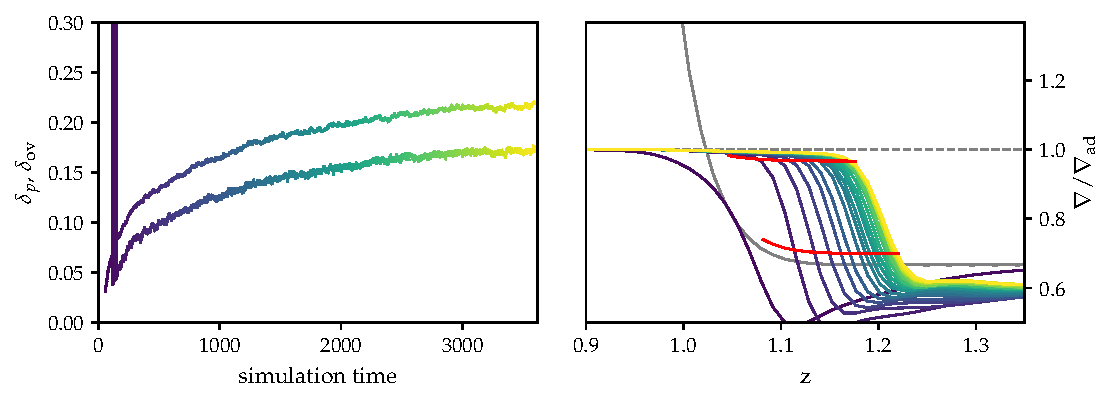
\includegraphics[width=\textwidth]{time_evolution.pdf}
\caption{
(Left top panel) Displayed is a trace of the PZ depth ($\delta_{0.5}$) vs.~time, with convective freefall time units on the bottom x-axis and thermal diffusion time units of the background $k$ in the radiative zone on the upper x-axis.
We also display the time evolution of $f$ (Left middle panel, defined in Eqn.~\ref{eqn:f_defn}) and $\xi$ (Left bottom panel, defined in Eqn.~\ref{eqn:xi_defn}).
The vertical lines in the left three panels show when the time trace first converges to within 1\% of its final value, which is denoted by a solid horizontal line.
(Right panel) The vertical profile of $\justgrad/\gradad$ is plotted against height at regular time intervals.
The line color denotes the time, according to the time traces in the left panels.
The constant value of $\gradad$ is denoted by the horizontal dashed grey line, and the value of $\gradrad$ is denoted by the solid grey line.
The location of the Schwarzschild convective boundary is displayed as a vertical dashed black line and denotes the place where $\gradad = \gradrad$.
The top of the penetration zone departure points are plotted over the profile evolution ($\delta_{0.1}$ and $\delta_{0.9}$ as red lines, $\delta_{0.5}$ as black lines).
\label{fig:time_evolution}
}
\end{figure}

In Fig.~\ref{fig:time_evolution}, we show the time evolution of a Case I (discontinuous conductivity) simulation with $\mR = 400$, $\mS = 10^3$, and $\mP_D = 4$ whose initial conditions roughly set $\justgrad = \gradad$ in the convection zone ($z \lesssim 1$) and $\justgrad = \gradrad$ in the radiative zone ($z \gtrsim 1)$.
In the top left panel, we display the measured extent of the penetrative region $\delta_{\rm{0.5}}$ vs.~time.
This region initially grows quickly over hundreds of freefall times, but this evolution slows down as the convective dynamics establish themselves and the final equilibration takes tens of thousands of convective overturn (freefall) times.
We note that this long evolution is extremely computationally costly; for this modest simulation (256x64$^2$ coefficients), this evolution represents roughly 20 days of evolution on 1024 cores for a total of $\sim$2.5 million cpu-hours.
It is not feasible to perform simulations of this length for a full parameter space study, and so we use smarter initial conditions and tricks to accelerate the evolution (see appendix \ref{app:accelerated_evolution} for details) for the bulk of the simulations in this work.

The evolution of the other parameters in our theory ($f$, $\xi$) are shown in the middle and bottom left panels of Fig.~\ref{fig:time_evolution}.
We plot the rolling mean, averaged over 1000 freefall time units. 
We see that the values of $f$ and $\xi$ reach their final values ($f \approx 0.67$, $\xi \approx 0.55$) faster than the penetration zone evolves to its full depth.
We quantify this by plotting a vertical line in each of the left three panels which corresponds to the first time in which the time-evolving average converges to within 1\% of the mean final value (calculated over the last 1000 freefall times of the simulation and plotted as a grey horizontal line).

In the right panel of Fig.~\ref{fig:time_evolution}, we display the realized profile of $\justgrad/\gradad$ in our simulations at regular time intervals (where the color of the profiles corresponds to time, as in the left panels).
$\gradad$ is plotted as a dashed horizontal line while $\gradrad$ is plotted as a grey solid line which decreases with height around $z \approx 1$ and satures to a constant above $z \gtrsim 1.1$.
The location of the Schwarzschild boundary, $L_s$, is overplotted as a black vertical dashed line and does not evolve over the course of the simulation.
We note that the Schwarzschild boundary does not move over the course of our simulation, so the extention of the convection zone past this point is true penetration and not the result of entrainment-induced changes in the Schwarzschild (or Ledoux) convective boundaries \citep[as studied in e.g.,][]{horst_etal_2021}.
The traces of $\delta_{0.1}$ and $\delta_{0.9}$ are plotted as red lines while that of $\delta_{0.5}$ is plotted as a black line.
We can see that the fast initial evolution establishes a sizeable PZ (denoted by purple $\justgrad$ profiles), but its final equilibration slows down (indicated by the separation between the profiles decreasing over time).
This occurs in part because the flattening of $\justgrad < \gradrad$ above the penetrative zone increases the effective value of $N^2$ and thus the stiffness at the PZ-RZ boundary.

\begin{figure}[t!]
\centering
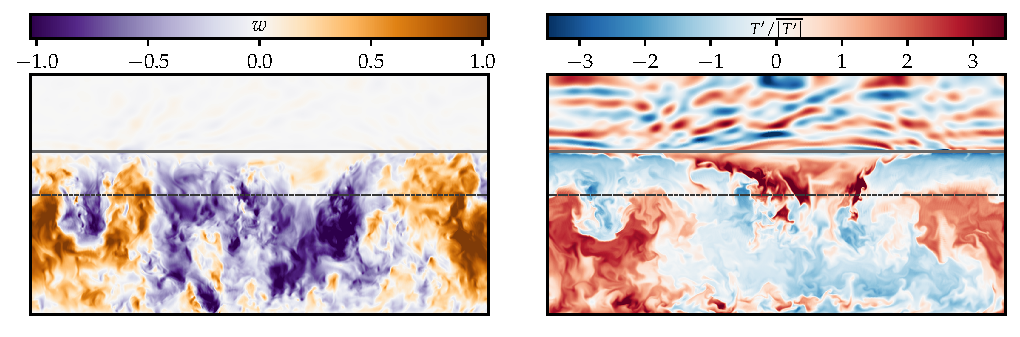
\includegraphics[width=\textwidth]{vertical_dynamics_panels.pdf}
\caption{
Displayed is an instantaneous snapshot of dynamics in a vertical slice through the simulation with $\mR = 6.4 \times 10^3$, $\mP_D = 4$ and $\mS = 10^3$.
In both panels, the nominal Schwarzschild boundary of the convection zone where $\gradad = \gradrad$ is displayed as a dashed horizontal line, and the top of the penetrative zone ($\delta_{0.1}$) is shown by a solid horizontal line.
(Left) The vertical velocity is shown; orange convective upflows extend far past the Schwarzschild boundary of the convection zone but stop abruptly where $\justgrad$ departs from $\gradad$.
(Right) Temperature fluctuations are shown, normalized by their average magnitude at each height in order to clearly display all dynamical features.
Unlike the vertical velocity, $T'$ shows distinctly different behavior in the CZ and PZ, switching sign at the Schwarzschild boundary of the convection zone.
\label{fig:vertical_dynamics_panels}
}
\end{figure}

In Fig.~\ref{fig:vertical_dynamics_panels}, we display instantaneous vertical slices through a turbulent simulation with $\mR = 6.4 \times 10^3$, $\mP_D = 4$ and $\mS = 10^3$ with a coefficient resolution of 384$^3$ in an equilibrated state.
We see that strong convective dynamics (viewed in the left vertical velocity panel) extend beyond the Schwarzschild boundary of the convection zone (horizontal dashed grey line) into a penetration zone.
Above the PZ, there is a dynamically distinct stable radiative zone with negligible vertical velocity (above the solid horizontal line).
On the right, we see that hot upwellings in the convective dynamics are turned into cold upwellings in the PZ as a result of effective cooling from the sharp change in $k$ around the Schwarzschild boundary of the convection zone.
These upwellings impinge upon the stable radiative zone and excite gravity waves, but our focus in this work is on the nature of the PZ where convective velocities and temperature anomalies are oppositely signed.


\subsection{Dependence on $\mP$}

We find that the depth of the penetration zone is strongly dependent on $\mP$.
In the upper two panels of Fig.~\ref{fig:parameters_vs_p}, we plot measured values of the penetration depth ($\delta_{0.1}$, $\delta_{0.5}$, $\delta_{0.9}$ from Eq.~\ref{eqn:delta_p_measures}) from Case I simulations (discontinuous $k$, upper left) and Case II simulations (discontinuous $\partial_z k$, upper right).
We find that the leading-order $\mP$ scaling predictions of Eqns.~\ref{eqn:discontinuous_prediction} \& \ref{eqn:linear_prediction} describe the data extremely well (orange lines).
At small values of $\mP$ we see somewhat weaker scalings than these predictions; this is a numerical artifact caused by the fact that the profiles of $k$ and $\partial_z k$ are not truly discontinuous but jump from one value in the CZ to another in the RZ over a finite width (See e.g., the $\gradrad$ profile in Fig.~\ref{fig:time_evolution}).
At large values of $\mP$, penetration depths begin to fall off of these predicted scaling laws, which makes sense: in this regime, dissipation dominates over buoyancy in the PZ and the PZ depths are saturating.

In the middle and bottom panels of Fig.~\ref{fig:parameters_vs_p}, we plot average values of $f$ (middle panels) and $\xi$ (bottom panels) from our theory.
These values are respectively defined in Eqns.~\ref{eqn:f_defn} \& \ref{eqn:xi_defn}.
We find that $f$ has slightly smaller values in the discontinuous-$k$ simulations (left) than in the discontinuous-$\partial_z k$ simulations (right).
We measure characteristic values of $f \in [0.6, 0.9]$, signifying that 60-90\% of the buoyant work is balanced by dissipation in the convection zone, depending on the simulation.
In general we find a trend in which $f$ and $\xi$ are weakly inversely proportional to $\mP$ in some way.
This likely relates to the changing nature of the PZ as a function of $\mP$.
When $\mP \ll 1$, $\delp \rightarrow 0$ and the PZ is essentially an abrupt boundary layer at the top of the CZ.
Convective motions run into an abrupt wall and fall off sharply, leading to higher values of $\xi$.
This wall-like nature of the PZ pushes flows sideways and we find that the changes in $f$ can largely be explained by increased velocities within the CZ as $\mP$ decreases.
In the case whree $\mP \gg 1$, $\delp$ becomes large and the PZ becomes similar in nature to the one shown in Fig.~\ref{fig:vertical_dynamics_panels}.
Here the PZ acts as a large extension of the convection zone in which convective motions slowly brake under their own buoyancy.
$\xi$ decreases in value as the dissipation profile falls off smoothly with height and $f$ decreases in value as the dynamics in the PZ become dominated by dissipation.
(TODO: think about this more)


\begin{figure}[t!]
\centering
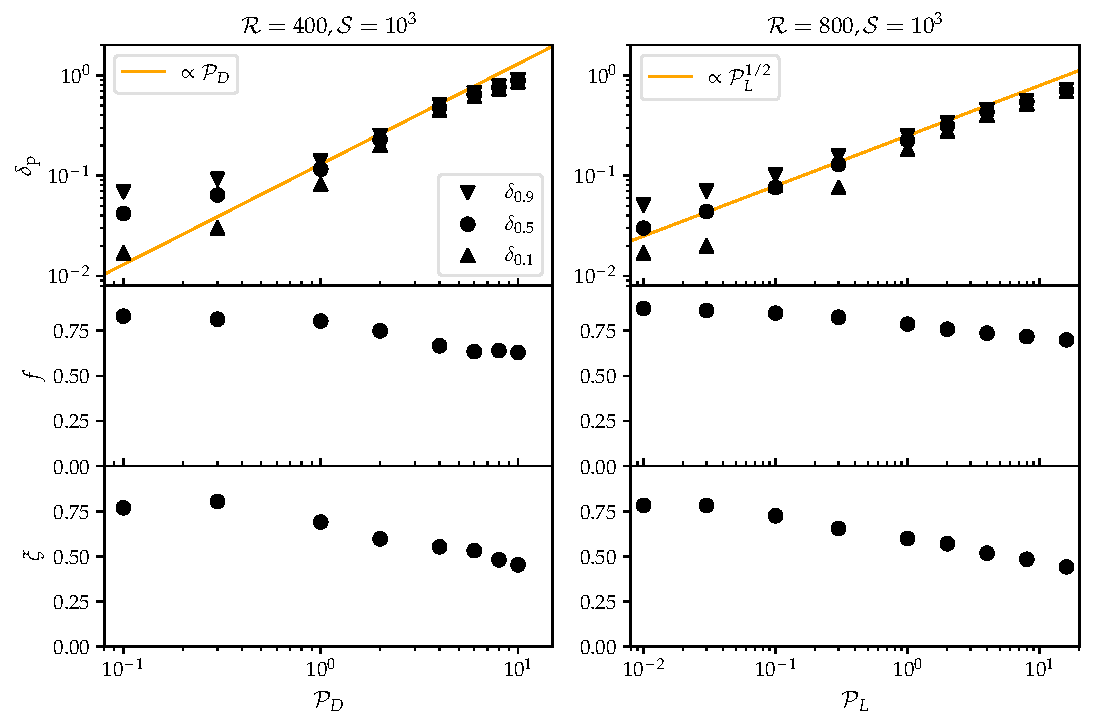
\includegraphics[width=\textwidth]{parameters_vs_p.pdf}
\caption{
Results from simulations with a Schwarzschild boundary characterized by a discontinuous conductivity (Left, $k$ defined by Eqn.~\ref{eqn:sim_discontinuous_k}) and with a discontinuous conductivity gradient (Right, $k$ defined by Eqn.~\ref{eqn:sim_discontinuous_k}).
The top panels show the measured penetration depths according to Eqn.~\ref{eqn:delta_p_measures}.
The discontinuous penetration depths (upper left) vary roughly linearly with $\mP$, in line with the prediction of Eqn.~\ref{eqn:discontinuous_prediction}.
The discontinuous-gradient penetration depths (upper right) vary roughly like $\sqrt{\mP}$, in line with the prediction of Eqn.~\ref{eqn:linear_prediction}.
In the middle panels, we measure the evolved value of $f$ according to Eqn.~\ref{eqn:f_defn}.
We generally find values of $f \in [0.5, 0.9]$, and changes in $f$ are secondary to changes in $\mP$ for determining penetration depths.
In the bottom panels, we measure the evolved values of $\xi$ according to Eqn.~\ref{eqn:xi_defn}.
We find characteristic values of $\xi \in [0.5, 0.75]$, suggesting that the falloff of the $\bar{\Phi}$ in the PZ is well described by a linear function (at high $\mP$ when $\xi = 1/2$), or by a cubic function (at low $\mP$ when $\xi \approx 3/4$).
\label{fig:parameters_vs_p}
}
\end{figure}

\subsection{Dependence on $\mS$}

We find that the depth of the penetration zone is weakly dependent on $\mS$.
In the left panel of Fig.~\ref{fig:parameters_vs_s}, we plot the penetration depth of a few discontinuous-$k$ simulations with $\mP_D = 4$ and $\mR = 400$ but with different values of $\mS$.
We find that the mean penetration depth $\delta_{0.5}$ varies only weakly with changing $\mS$, but that the values of $\delta_{0.1}$ and $\delta_{0.9}$ vary somewhat strongly.
In other words, the smooth transition region in which $\justgrad$ varies from $\gradad$ in the PZ to $\gradrad$ in the RZ becomes narrower as $\mS$ becomes smaller.
To quantify this effect, we plot $\delta_{0.9} - \delta_{0.1}$ in the righthand panel of Fig.~\ref{fig:parameters_vs_s}.
We find that the width of this region roughly varies according to a $\mS^{-1/2}$ scaling law, which is reminiscent of the pure-overshoot laws described by \citet{korre_etal_2019}.
This suggests that the evolved profile of a convecting region can be described by a penetration zone (described by e.g., $\mP$, $f$, and $\xi$) with a thin overshooting region (described by $\mS$) within the transition between the PZ and RZ.

We note briefly that if the enstrophy, $\omega^2$ in the convection zone exceeded the value of the square buoyancy frequency $N^2$ in the radiative zone, the gravity waves in the RZ became nonlinear.
As a result, we have restricted the simulations in this study to relatively large (yet modest compared to astrophysical values) of $10^{2} \leq \mS < 10^4$ in order to ensure $N^2 > \omega^2$.

\begin{figure}[t!]
\centering
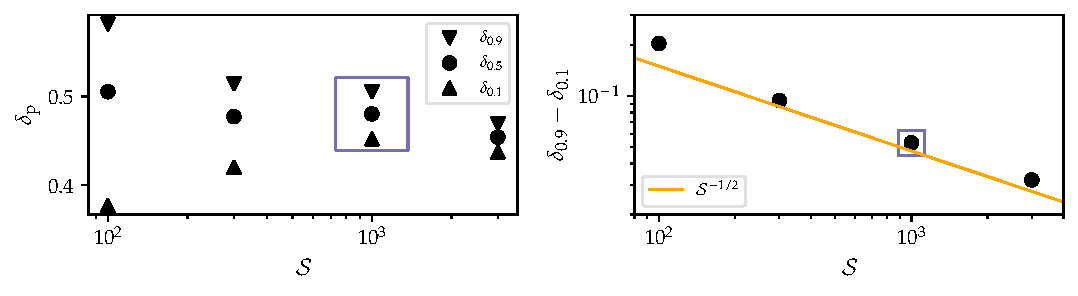
\includegraphics{parameters_vs_s.pdf}
\caption{
(Left panel) Penetration depths are shown as a function of stiffness for simulations with a discontinuous conductivity.
While the width of the transition layer from the adiabatic PZ to the stable RZ shrinks as a function of $\mS$, the mean penetration depth ($\delta_{0.5}$) is roughly constant.
(Right panel) The width of the thermal transition layer ($\delta_{0.9} - \delta_{0.1}$) is shown as a function of stiffness.
We roughly observe a $\mS^{-1/2}$ scaling, similar to that expected by e.g., \citet{korre_etal_2019}.
\label{fig:parameters_vs_s}
}
\end{figure}

\subsection{Dependence on $\mR$}

We find that the depth of the penetration zone is weakly dependent on $\mR$.
In the upper left panel of Fig.~\ref{fig:parameters_vs_re}, we find a logarithmic decrease in the penetration depth $\delta_{0.5}$ with the Reynolds number.
In order to understand how this could happen at fixed $\mP$, we plot the output values of our parameterized values $f$ (upper middle) and $\xi$ (upper right).
We find that $f$ increases with increases $\mR$, but is perhaps leveling off.
We find that $\xi$ does not increase strongly with $\mR$ except for in the case of laminar simulations with $\mR < 200$.
Indeed, we see in the bottom left panel that this variation of $\delp$ with $\mR$ can equally be seen as a variation of $\delp$ with $f$.
We find that this is true both for simulations with stress-free lower boundary (open symbols, SF) and for no-slip lower boundaries (closed symbols, NS).

In order to understand this better, we note that, at least in the SF simulations, the dissipation can roughly be modeled as a constant value in the CZ and zero in the viscous boundary layer (in the NS case, the dissipation becomes a maximum in the boundary layer).
This means that we can model the dissipation in the $f$ definition (Eqn.~\ref{eqn:f_defn}) as
\begin{equation}
\int \bar{\Phi} dz = C ( L_s - \delta_\nu ),
\end{equation}
where $C$ is a constant dissipation value in the CZ and $\delta_\nu$ is the boundary layer depth.
In other words, under this model, we expect the dissipation, and thus $f$, to vary linearly with the viscous boundary layer depth.
Indeed, we find this to roughly be the case for the stress-free simulations in the bottom middle panel of Fig.~\ref{fig:parameters_vs_re}.
We find that the NS simulations show a more complex increase as $\delta_\nu \rightarrow 0$ due to the fact that dissipation is maximized in the boundary layer and its magnitude there varies with $\mR$.
Regardless, we find that the depth of the viscous boundary layer follows classical scaling laws from Rayleigh-B\'{e}nard convection \citep{ahlers_etal_2009, goluskin2016}, as shown in the bottom right panel of Fig.~\ref{fig:parameters_vs_re}, and so we anticipate that the value of $f$ should saturate as $\mR$ increases into the astrophysical regime.

Unfortunately, we are limited by the long evolutionary timescales of these simulations (see Fig.~\ref{fig:time_evolution}), so we cannot extend our study to more turbulent simulations and higher values of $\mR$ than the ones shown here.
We are only able to run the NS simulation at $\mR = 6.4 \times 10^3$ for a few hundred freefall times, and so cannot investigate the nature of these trends further.
However, the link between $\delta_{0.5}$ and $f$ and the link between $f$ and $\delta_\nu$ -- both of which are effects we largely understand -- give us hope that PZ depths should saturate at high $\mR$.


\begin{figure}[t!]
\centering
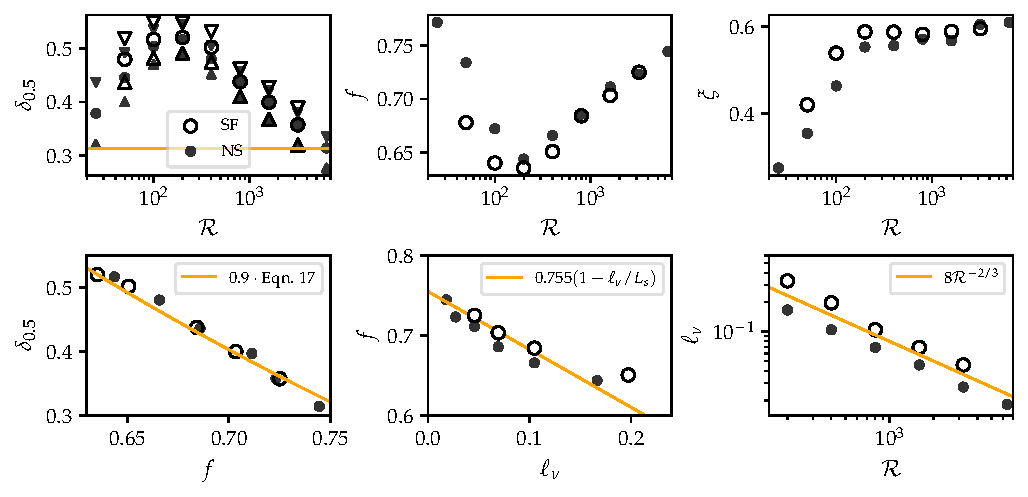
\includegraphics{parameters_vs_re.pdf}
\caption{
(Upper left panel) Penetration depths are shown as a function of increasing Reynolds number ($\mR$) for simulations with a discontinuous conductivity.
We plot results both for cases with stress-free boundary conditions (SF) and no-slip boundary conditions (NS).
In both cases, we see a roughly logarithmic decrease of $\delp$ with $\mR$.
(Upper middle panel) We similarly see increases in the value of $f$ with $\mR$, although perhaps this measurement is leveling off at high values of $\mR$.
(Upper right panel) We do not see large changes in the value of $\xi$ as $\mR$ increases, suggesting that the nature of dissipation in the PZ is not appreciably changing.
(Lower left panel) In summary, we see a strong correlation between $\delta_{0.5}$ and $f$.
(Lower middle panel) Changes in $f$ are roughly linearly proportional to the depth of the viscous boundary layer, $\delta_\nu$, at the bottom of the domain, at least for the open-circle SF cases.
This makes sense, as more of the convective domain is available for the convective flows to dissipate energy.
(Lower right panel) The viscous boundary layer follows a classical scaling laws seen in Rayleigh-B\'{e}nard convection, and so we anticipate that the trend in $\delta_{0.5}$ vs $\mR$ should saturate as $\delta_{\nu} \rightarrow 0$ and $f$ saturates.
\label{fig:parameters_vs_re}
}
\end{figure}


\section{A modified solar model}
\label{sec:solar_model}
Our simulation results present a strong case for the validity of a flux- and dissipation-based model of convective penetration, similar to those considered by \citet{zahn1991} and \citet{roxburgh1989}.
In general, out of the simulations presented in this work, we expect the simulation with $\mP_L = 1$ (a linear radiative conductivity profile) to be the most representative of conditions near a stellar convective boundary.
In this simulation, we found $f \approx 0.8$ and $\xi \approx 0.6$; the results of Fig.~\ref{fig:parameters_vs_re} suggest that $f$ could increase by $\sim 0.1$ as $\mR$ increases into the stellar regime but $\xi$ probably doesn't change much.
As such, we take $f \approx 0.9$ and $\xi \approx 0.6$ as first-guess values for our theory of convective penetration in stellar regimes.
These values should of course be confirmed and tuned in more realistic stellar settings which include spherical geometry and realistic density stratifications.

In spherical geometry, if the horizontal averages of Eqn.~\ref{eqn:integral_constraint} are replaced with horizontal averages, the relevant integral constraint for convective penetration can be described in terms of the convective luminosity,
\begin{equation}
\int |\alpha| g L_{\rm{conv}}\,dr =   \int 4\pi \rho_0 r^2\bar{\Phi}\,dr,
\end{equation}
where $L_{\rm{conv}} = 4\pi\rho_0 r^2 \bar{F_{\rm{conv}}}$ and $r$ is the radial coordinate.
Following the same logic as Sct.~\ref{sec:theory}, the equivalent of Eqn.~\ref{eqn:theory_frac} is
\begin{equation}
-\frac{\int_{\rm{PZ}} L_{\rm{conv}}\,dr}{\int_{\rm{CZ}} L_{\rm{conv}}\,dr} + f \xi \frac{(1 + [\delp/r_s])^3 - 1}{1 - (r_{\rm{CZ}}/r_s)^3} = (1 - f),
\end{equation}
where the CZ integral is taken from $r_{\rm{CZ}}$ to $r_s$ and the PZ integral is taken from $r_s$ to $r_s + \delp$, and the extra factors in the $\xi$ term come from accounting for spherical geometry.
Linearly truncating a Taylor expansion of this geometric term around $\delp/r_s \approx 0$, we retrieve
\begin{equation}
-\frac{\int_{\rm{PZ}} L_{\rm{conv}}\,dr}{\int_{\rm{CZ}} L_{\rm{conv}}\,dr} + 3 f \xi \frac{\delp}{r_s}(1 - [r_{\rm{CZ}}/r_s]^3)^{-1} \approx (1 - f).
\label{eqn:mesa_eqn}
\end{equation}
In the case of solar convection, $r_{\rm{CZ}} = R_{\odot}$, $r_s \approx 0.7R_{\odot}$ (the Schwarzschild-defined bottom of the CZ), and $\delp$ is some (negative) value so that the penetration zone ends at $r_s + \delp$.

We ran a MESA solar model using Eqn.~\ref{eqn:mesa_eqn} with $f = 0.9$ and $\xi = 0.6$ to determine an extremely rough first-estimate of how the dissipative treatment presented in this work might adjust a familiar stellar model.
The details of this implementation are laid out in Appendix \ref{app:mesa}.
We of course note that the work that we presented here is done under the incompressible approximation and does not include the many complications of stellar convection like density stratification, sphericity, rotation, magnetism, etc.
We present this as a proof of concept and to inspire further work.

In Fig.~\ref{} we display the profile of X quantity at the base of a solar model using a penetrative zone (as described above) and using X classical prescription.
Note the differences in this thing and that thing.

TODO: Implement this in MESA, and make a simple figure comparing some solar profiles near the base of the CZ!

We find a convection zone which extends an additional $X H_p$ beneath the nominal Schwarzschild base of the convection zone.
Past work has suggested from observations that the maximum depth of such an extended adiabatic region should be limited to $0.05 H_p$, which is smaller than what is found in our model \citep[see e.g., section 7.2.1 of][]{basu2016}.
However, our results here are in line with the recent simulations of \citet{kapyla2019}, which suggest an overshooting depth of $0.2 H_p$ at the base of the solar convection zone.
We hope to improve this model and stuff in future work, please hang out with us and make it better.


\section{Discussion}
\label{sec:discussion}
In this work, we used an integral constraint \citep[reminiscent of][]{roxburgh1989} and flux-based arguments \citep[similar to][]{zahn1991} to derive a parameterization of convective penetration according to the convective flux and viscous dissipation.
We parameterized the viscous dissipation into a bulk-CZ portion ($f$) and a portion in the extended penetrative region ($\xi$), and derived predictions for how the depth of a penetrative region, $\delp$, should scale with these parameters and a new flux-based ``penetration parameter'' $\mP$.
We designed and analyzed two sets of simulations which showed good agreement with these theoretical predictions.
We furthermore examined briefly what the impliciations of this theory could be for a simple solar model.
Our results suggest that stellar convection zones should be bounded by appreciably large penetration zones.
In extreme cases, we observe penetration zones which are as large as the convection zones they accompany; however, for realistic stellar values ($\mP \approx 1$), we find that they may be as large as 20-30\% of the convective zone length scale ($\sim$the mixing length).

The simulations we presented in this work were the simplest possible simulations to try to test the basic tenets of our theory.
In particular, they demonstrate that the shape of the flux near the convective boundary and the viscous dissipation together fully determine the depth of the penetration zone.
The precise values of the parameters $f$ and $\xi$ achieved in natural, turbulent, fully compressible, spherical stellar convection may be different from those presented in e.g., Fig.~\ref{fig:parameters_vs_p} here.
Future work should aim to understand how these parameters change when these realistic effects are taken into account.

Furthermore, it is important to note that stellar opacities, and thus stellar conductivities, are functions of thermodynamic variables rather than radial location.
As a result, the formation of a penetration zone will in turn affect the conductivity profile and $\gradrad$, which will in turn affect the estimate of how deep the penetration zone should be.
Future studies should follow e.g., \citet{kapyla_etal_2017} and implement realistic opacity profiles which evolve self-consistently with the thermodynamic state in order to understand how these effects feedback into one another.

An additional complication is that stellar fluid dynamics exist in the regime of Pr$\,\ll1$ \citep{garaud2021}.
Dynamics in this regime may be different from those in the regime of Pr $\lesssim 1$ that we studied here, which in theory could affect $f$ and $\xi$.
Recently, \citet{kapyla2021} found that convective flows exhibited more penetration at low Pr than high Pr.
Future work should aim to understand whether $f$ and $\xi$ depend strongly on $\Pran$ in the turbulent regime.

Two other interesting complications in stellar contexts are rotation and magnetism.
In the rapidly rotating limit, rotation creates quasi-two-dimensional flows, which could affect the length scales on which dissipation acts and thus modify $f$.
Furthermore, magnetism adds an additional ohmic dissipation term, which could in theory drastically change our hydrodynamical measurement of $f$.

Finally, we note that our work here assumes a uniform composition through the convective and radiative region.
Frequently within stars, convective boundaries coincide with discontinuities in composition profiles \citep{salaris_cassisi_2017}.
Future work should also aim to determine if stabilizing composition gradients can prevent the formation of penetration zones seen here (as in Fig.~\ref{fig:time_evolution}).

In summary, we have unified \citet{roxburgh1989}'s integral constraint with \citet{zahn1991}'s theory of flux-dependent penetration into a parameterized theory of convective penetration.
We tested this theory with simulations and found good agreement between the theory and our simulations.
In future work, we will aim to more robustly implement this theory into MESA and test some of the complicating factors we discussed here.





\begin{acknowledgments}
We'd like to thank Keaton Burns, Matt Browning, Matteo Cantiello and Kyle Augustson for useful discussions and questions which improved the content of this manuscript.
TODO thank Nordita program.
EHA is funded as a CIERA Postdoctoral fellow and would like to thank CIERA and Northwestern University. 
Computations were conducted with support from the NASA High End Computing (HEC) Program through the NASA Advanced Supercomputing (NAS) Division at Ames Research Center on Pleiades with allocation GID s2276.
\end{acknowledgments}


\appendix

\section{Accelerated Evolution}
\label{app:accelerated_evolution}
As demonstrated in Fig.~\ref{fig:time_evolution}, the time evolution of simulations which start from a state based on the Schwarzschild criterion can be prohibitively long.
In \citet{anders_etal_2018}, we explored the long time evolution of simple convective simulations and found that fast-forwarding the evolution of a convective simulation's internal energy and thermal structure can be done accurately.
This can be done because the convective dynamics converge rapidly even if the thermal profile converges slowly.
This same separation of scales is observed in the top and bottom left panels of Fig.~\ref{fig:time_evolution} in this work, and so similar techniques should be applicable.

In this work, we accelerate the evolution of of our simulations in order to more quickly determine the final size of the evolved penetration zones according to the following algorithm.
\begin{enumerate}
\item Once a simulation has a volume-averaged Reynolds number greater than 1, we wait 10 freefall times to allow dynamical transients to pass.
\item We measure the departure points ($\delta_{0.1}$, $\delta_{0.5}$, $\delta_{0.9}$) every freefall time, and store this information for 30 freefall times.
\item We linearly fit each of the departure points' evolution against time using NumPy's \texttt{polyfit} function.
We assume that convective motions influence $\delta_{0.1}$ and $\delta_{0.5}$ more strongly than $\delta_{0.9}$.
We measure the time-evolution of the convective front $\frac{d \delp}{dt}$ by averaging the slope of the linear fits for $\delta_{0.1}$ and $\delta_{0.5}$.
\item We take a large ``time step'' of size $\tau_{\rm{AE}}$ forward.
We calculate $\Delta \delta_p = \tau_{\rm{AE}} \frac{d \delp}{dt}$.
\begin{itemize}
\item If $\Delta \delta_p < 0.005$, we erase the first 15 time units worth of departure point measures and return to step 2 for 15 time units.
\item  If $\Delta \delta_p$ is large, we adjust the top of the PZ by setting $\delta_{0.5,\rm{new}} = \angles{\delta_{0.5}}_t + \Delta \delta_p$ (angles represent a time average).
If $|\Delta \delta_p| > 0.05$, we limit its value to 0.05.
We calculate the width of the thermal adjustment layer $d_w$ as the minimum of $\angles{\delta_{0.9} - \delta_{0.5}}_t$ and $\angles{\delta_{0.5} - \delta_{0.1}}_t$.
We adjust the mean temperature gradient to
\begin{equation}
\partial_z \overline{T} = -\gradad - H(z; \delta_{\rm{0.5,\rm{new}}}, d_w) \Delta\justgrad,
\label{eqn:initial_grad}
\end{equation}
where $H$ is defined in Eqn.~\ref{eqn:heaviside} and $\Delta\justgrad = \gradrad - \gradad$.
We also multiply the temperature perturbations and full convective velocity field by $(1 - H(z; 1, 0.05))$.
This sets all fluctuations above the nominal Schwarzschild convection zone to zero, thereby avoiding any strange dynamical transients caused by the the old dynamics at the radiative-convective boundary (which has moved as a result of this process).
\end{itemize}
\item We restart from step 1.
\end{enumerate}
In general, we start our simulations with an initial profile according to Eqn.~\ref{eqn:initial_grad} with a value $\delta_{0.5,\rm{new}} \geq 0$.
If a simulation returns to step 2 from step 4 ten times over the course of its evolution, we assume that it has converged near its answer, stop this iterative loop, and allow the simulation to timestep normally.
Additionally, in some simulations, we ensure that this process occurs no more than 25 times.
This process effectively removes the long diffusive thermal evolution on display in the middle left panel of Fig.~\ref{fig:time_evolution} by immediately setting the mean temperature profile to the radiative profile above the PZ.

In Fig.~\ref{fig:AE_time_figure}, we display the time evolution of $\delp/\tilde{L_s}$ and $\angles{f}$ in the $\mP_D = [1,2,4]$ simulations using black lines.
We overplot the evolution of simulations which use this accelerated evolution procedure using orange and green lines.
For the orange-line simulations, we use initial conditions which specify a value of $\delp$ that is smaller than the expected evolved value of $\delp$.
For the purple-line simulations, we use initial conditions which specify a value of $\delp$ that is larger than the expected evolve value.
Regardless of our choice of initial condition, we find that this AE procedure quickly evolves our simulations to within a few percent of the final value.
If these simulations are not in a stationary state after this procedure, we timestep them straightforwardly until we are satisfied that they have converged.

\begin{figure}[t!]
\centering
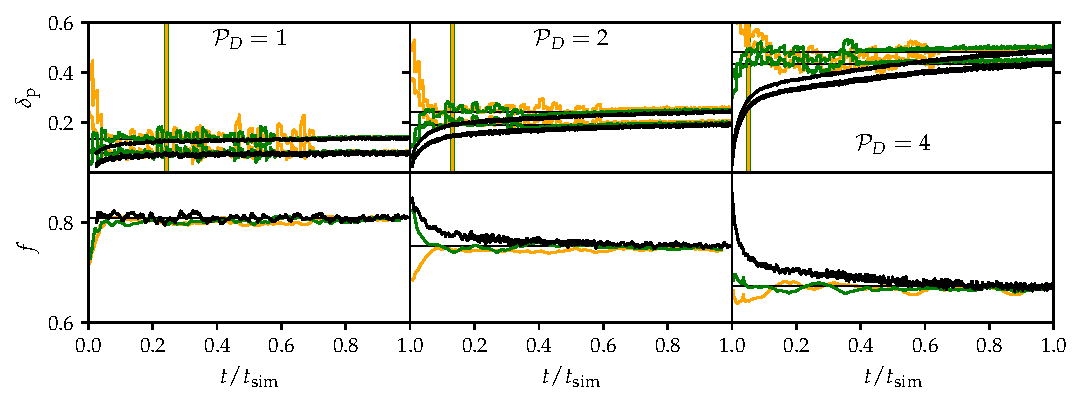
\includegraphics[width=\textwidth]{AE_time_figure.pdf}
\caption{
\label{fig:AE_time_figure}
(top row) Time traces of $\delta_p/\tilde{L_s}$ for simulations which are computed using (black lines) standard timestepping, (green lines) accelerated evolution with large initial values of $\delp$, and (orange lines) accelerated evolution with small initial values of $\delp$.
Accelerated evolution timesteps can be see as discontinuities in the $\delp/\tilde{L_s}$ trace.
Once the procedure gets to within a few percent of the appropriate value, any large steps away from the ``correct'' solution are quickly reversed.
(Bottom row) Same as top row, but where $\angles{f}$ is being shown.
}
\end{figure}



\section{Table of simulation parameters}
\label{app:simulation_table}


\section{MESA implementation}
\label{app:mesa}
We now examine briefly how our theory modifies a simple structure model of the Sun.
We implement a simple prescription of convective penetration in MESA \citep{paxton_etal_2013} as follows:
\begin{enumerate}
\item Find the radial location of the radiative-convective boundary according to the Schwarzschild criterion, $r_{\rm{RCB}}$.
Also evaluate the value of the mixing length $\ell$ at that location.
\item Integrate the magnitude of the convective luminosity within the convection zone, $L_{\rm{CZ}} = \int_{r_{\rm{RCB}}}^{r_{\rm{RCB}} + \ell} L_{\rm{conv}} dr$.
\item Following Eqn.~\ref{eqn:theory_fraction} and the measured values for $f$ in Eqn.~\ref{eqn:fit_f_values}, integrate $L_{\rm{PZ}} = \int_{r_{\rm{RCB}}}^{r_{\rm{RCB}} + \delp} (L_{\rm{rad}} - L_{\rm{rad,ad}}) dr$, where $L_{\rm{rad}}$ is the radiative luminosity carried by $\gradrad$ and $L_{\rm{rad,ad}}$ is the radiative luminosity carried by $\gradad$.
We determine the value of $\delp$ according to Eqn.~\ref{eqn:theory_fraction} so that
\begin{equation}
L_{\rm{PZ}} = (1 - f)L_{\rm{CZ}},
\label{eqn:mesa_equation}
\end{equation}
with an initial guess of $f = 0.9$.
\item Override the value of $\justgrad$ in the MESA solver to set $\justgrad = \gradad$ from $r_{\rm{RCB}}$ to $r_{\rm{RCB}} - \delta_p$.
\item Mix within this new convection zone by setting the convective velocities according to the average convective luminosity in the penetration zone, $4\pi r^2 \rho v^3 \sim L_{\rm{PZ}}$.
\end{enumerate}





\bibliographystyle{aasjournal}
\bibliography{biblio}
\end{document}
